\title{Midterm 2 for Algebra-based Physics}
\author{Dr. Jordan Hanson - Whittier College Dept. of Physics and Astronomy}
\date{\today}
\documentclass[10pt]{article}
\usepackage[margin=1.5cm]{geometry}
\usepackage{outlines}
\usepackage{graphicx}
\usepackage{amsmath}

\begin{document}
\maketitle

\section{Memory Bank}

\begin{itemize}
\item Unit conversions: 1 km = 1000 m, 1 m = 100 cm, 1 hr = 3600 s, 1 year = $\pi \times 10^7$ s, 1 g/cm$^3$ = 1000 kg/m$^3$.
\item $\vec{x} = a \hat{i} + b\hat{j}$ ... Component form of a two-dimensional vector.
\item $|\vec{x}| = \sqrt{a^2+b^2}$ ... Pythagorean theorem for obtaining vector magnitude.
\item $\theta = \tan^{-1}(b/a)$ ... Obtaining the angle between vector and x-axis.
\item $a = |\vec{x}|\cos(\theta)$ ... Obtaining the x-component with trigonometry.
\item $b = |\vec{x}|\sin(\theta)$ ... Obtaining the y-component with trigonometry.
\item $x(t) = x_i + v t$ ... Velocity is the slope of position versus time.
\item $x(t) = \frac{1}{2} a t^2 + v_i t + x_i$ ... With constant acceleration, position is quadratic.  If $a=0$ this becomes the prior function.
\item $v(t) = v_i + a t$ ... With constant acceleration, acceleration is the slope of velocity.
\item $v^2 = v_i^2 + 2 a \Delta x$ ... The kinematic equation without time, assuming constant acceleration.
\item $\vec{F}_{net} = 0$ ... Newton's First Law, an object with no net force stays at constant velocity, or zero velocity.
\item $\vec{F}_{net} = m\vec{a}$ ... Newton's Second Law.
\item $\vec{F}_{AB} = -\vec{F}_{BA}$ ... Newton's Third Law.
\item $\vec{w} = - mg \hat{j}$ ... Weight force.
\item $\vec{N} = +mg\hat{j}$ ... Normal force, when the object is on a flat surface.
\item $N = mg\cos\theta$, $w_x = -mg\sin\theta$, $w_y = -mg\cos\theta$ ... Incline plane forces.
\item $f = \mu N$, $F_D = \frac{1}{2}C\rho A v^2$, $F_D = 6\pi r \eta v$ ... friction, drag in air, drag in viscous fluids.
\item $stress = Y \times strain$, or $F/A = Y (\Delta x / L)$ ... Young's Modulus and elasticity.
\item $s = r \theta$ ... Definition of a \textit{radian}, with arc length $s$ and angle $\theta$.
\item $v = r\omega$, $a = r\alpha$ ... Angular velocity, angular acceleration.
\item $a_C = v^2/r = r\omega^2$ ... Centripetal acceleration.
\item $F_C = m a_C = mv^2/r = mr\omega^2$ ... Centripetal force.
\item $\vec{F}_G = G m_1 m_2/r^2 ~~ \hat{r}$ ... Newton's Law of Gravity.
\end{itemize}

\section{Chapter 4: Dynamics, Force and Newton's Laws of Motion}

\begin{enumerate}
\item A $5\times 10^5$ kg rocket is accelerating straight up.  The thrusters produce an upward force of $1.25 \times 10^7$ N, and the force of air resistance is $4.5 \times 10^6$ N downward.  (a) Draw a free-body diagram including the weight of the rocket, the thrust, and air resistance.  (b) What is the rocket’s acceleration? \\ \vspace{2cm}
\item A football player with mass 70 kg pushes on a player with mass 90 kg.  (a) According to Newton's 3rd law, if the first player exerts a force of 700 N on the second player, what is the force the second player exerts on the first player? \\ \vspace{1cm}
\item A rocket sled is decelerated at a rate of 200 m/s$^2$, and it has a mass of 2000 kg.  There is a constant air resistance force of 1000 N.  What additional force is required to give the rocket the deceleration?  \\ \vspace{2cm}
\item A 76.0-kg person is being pulled away from a burning building as shown in Fig. \ref{fig:fire}.  (a) Draw a free-body diagram including the two tension vectors and the woman's weight.  (b) Write down an expression for $F_{net,x}$.  (c) Write down an expression for $F_{net,y}$.  (d) Assuming $\vec{F}_{net} = 0$, calculate the tension in the two ropes. \\ \vspace{2.5cm}
\begin{figure}[hb]
\centering
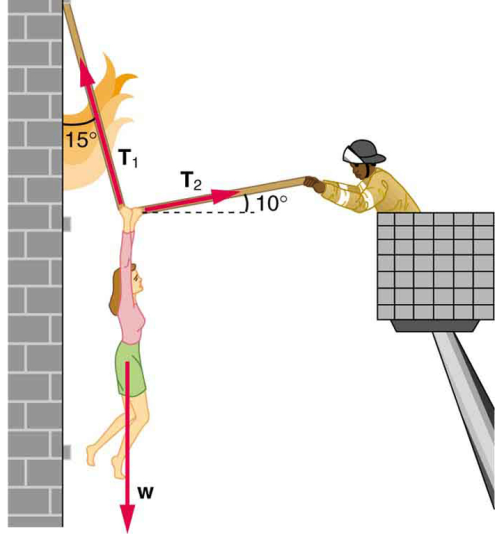
\includegraphics[width=0.35\textwidth]{fire.png}
\caption{\label{fig:fire} A person is pulled from a building using tension in a rope.}
\end{figure}
\end{enumerate}

\clearpage

\section{Chapter 5: Friction, Drag, and Elasticity}

\begin{enumerate}
\item Suppose you have a 120-kg wooden crate resting on a wood floor. The coefficients of static and kinetic friction are 0.5 and 0.3, respectively.  (a) What maximum force can you exert horizontally on the crate without moving it? (b) If you continue to exert this force once the crate starts to slip, what will the magnitude of its acceleration then be? \\ \vspace{2.0cm}
\item 
\begin{figure}[ht]
\centering
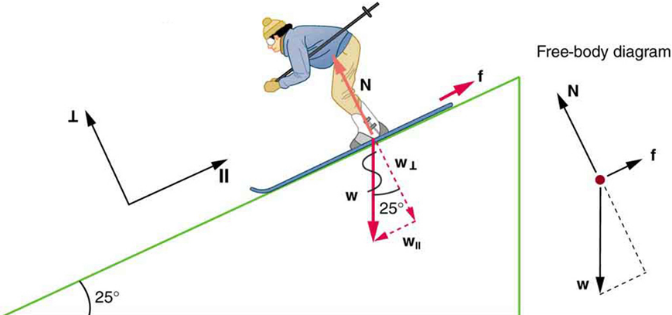
\includegraphics[width=0.5\textwidth]{ski.png}
\caption{\label{fig:ski} A skier slides down a slope.}
\end{figure}
Suppose a skier (Fig. \ref{fig:ski}) is sliding down a slope with an incline of 25 degrees.  If the coefficient of kinetic friction is 0.1, what is the skier's acceleration? \\ \vspace{2.0cm}
\item \textbf{Drag Force}.  Suppose the skier reaches a top speed of 40 m/s.  If his area is 0.75 m$^2$, the density of air is 1.225 kg m$^{-3}$, and $C = 0.75$, what is the magnitude of the drag force in Newtons?  \\ \vspace{2cm}
\item A mass of 2300 kg is place on top of a 10.0 m long wooden beam with radius of 4 cm. If the length of the beam decreases by 3 mm, what is the Young's modulus of the wood? \textit{Pay attention to the units}.  \\ \vspace{2cm}
\end{enumerate}

\section{Chapter 6: Uniform Circular Motion and Gravitation}

\begin{enumerate}
\item  A pitcher in baseball pitches a ball at 144 km per hour, and the ball rotates around his arm at a radius of 0.5 meters.  What is the angular velocity of the ball as he throws it, in radians per second? \\ \vspace{1cm}
\item What is the ideal banking angle for a gentle turn of 0.9 km radius on a highway with a 120 km per hour speed limit, assuming everyone travels at the limit? \\ \vspace{2cm}
\item Two race car drivers routinely navigate a turn as shown in Fig. \ref{fig:race}.  (a) Which path may be taken at a higher speed, if both paths correspond to the same force of friction and centripetal force? (b) Suppose path 1 has a radius of curvature of 400 m, and path 2 has a radius of curvature of 800 m.  The coefficient of friction is 1.0.  If the force of friction balances the centripetal force, what are the tangential velocities of each race car? \\ \vspace{1cm}
\begin{figure}[ht]
\centering
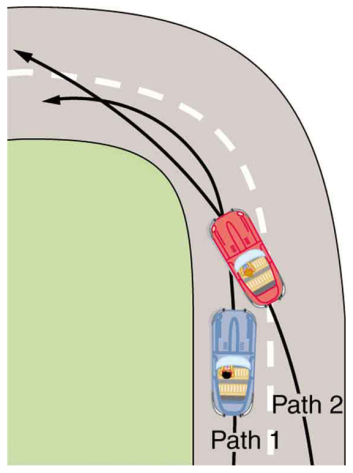
\includegraphics[width=0.25\textwidth]{race.png}
\caption{\label{fig:race} Two race cars take a turn at different radii of curvature.}
\end{figure}
\item \textbf{Two bonus points:} The existence of the dwarf planet Pluto was proposed based on irregularities in Neptune’s orbit. Pluto was subsequently discovered near its predicted position. But it now appears that the discovery was fortuitous, because Pluto is small and the irregularities in Neptune’s orbit were not well known. To illustrate that Pluto has a minor effect on the orbit of Neptune compared with the closest planet to Neptune, (a) calculate the acceleration due to gravity at Neptune due to Pluto when they are $4.5 \times 10^{12}$ m apart, as they are now.  The mass of Pluto is $1.4 \times 10^{22}$ kg.  (b) Now calculate the acceleration due to gravity at Neptune due to Uranus, presently about $2.5 \times 10^{12}$ m apart, and compare it with that due to Pluto.  The mass of Uranus is $8.62 \times 10^{25}$ kg. \\ \vspace{1cm}
\end{enumerate}

\end{document}